\documentclass[11pt, oneside]{article}   	% use "amsart" instead of "article" for AMSLaTeX format
\usepackage[utf8]{inputenc}
\usepackage{geometry}                			% See geometry.pdf to learn the layout options. There are lots.
\geometry{letterpaper}                   			% ... or a4paper or a5paper or ... 
%\geometry{landscape}                			% Activate for rotated page geometry
%\usepackage[parfill]{parskip}    			% Activate to begin paragraphs with an empty line rather than an indent
\usepackage{graphicx}							% Use pdf, png, jpg, or eps§ with pdflatex; use eps in DVI mode
																% TeX will automatically convert eps --> pdf in pdflatex		
\usepackage{amssymb}
\usepackage{listings}
\usepackage{xcolor}
\usepackage[export]{adjustbox}
\usepackage{booktabs}
\usepackage{float}
\usepackage{tikz}
\usepackage{pgfplots}
\usepgfplotslibrary{fillbetween}
\usetikzlibrary{patterns}
\pgfplotsset{compat=1.16}

\definecolor{codegreen}{rgb}{0,0.6,0}
\definecolor{codegray}{rgb}{0.5,0.5,0.5}
\definecolor{codepurple}{rgb}{0.58,0,0.82}
\definecolor{backcolour}{rgb}{0.95,0.95,0.92}

\lstdefinestyle{mystyle}{
	backgroundcolor=\color{backcolour},   
	commentstyle=\color{codegreen},
	keywordstyle=\color{magenta},
	numberstyle=\tiny\color{codegray},
	stringstyle=\color{codepurple},
	basicstyle=\ttfamily\footnotesize,
	breakatwhitespace=false,         
	breaklines=true,                 
	captionpos=b,                    
	keepspaces=true,                 
	numbers=left,                    
	numbersep=5pt,                  
	showspaces=false,                
	showstringspaces=false,
	showtabs=false,                  
	tabsize=2
}

\lstset{style=mystyle}

\title{Domain Testing}
\author{Zelin Cai, Patrick Silvestre}
\date{}

\begin{document}
\maketitle

\section{\texttt{ticketing\_module.py}}
\begin{lstlisting}[language=Python]
__author__ = "Zelin Cai, Patrick Silvestre"
__license__ = "MIT"


def ticketing_module(age, gender):
    if gender == "boy":
        if age < 6:
            return "rhyming"
        elif 7 < age < 10:
            return "storytelling"
        elif 11 < age < 15:
            return "quiz"
        elif 20 < age:
            return "poetry"
        else:
            return ""
    elif gender == "girl":
        if age < 6:
            return "rhyming"
        elif 7 < age < 10:
            return "drawing"
        elif 10 < age < 15:
            return "essay writing"
        elif 20 < age:
            return "poetry"
        else:
            return ""
    else:
        return ""
\end{lstlisting}
\newpage

%\section{\texttt{test\_ticketing\_module.py}}
%\begin{lstlisting}[language=Python]
%__author__ = "Zelin Cai, Patrick Silvestre"
%__license__ = "MIT"
%
%from ticketing_module import *
%import unittest
%
%class testInvalidValues(unittest.TestCase):
%    def test1(self):
%        actual_output = ticketing_module(10, "none")
%        expected_output = ""
%        self.assertEqual(actual_output, expected_output)
%
%class testBoy(unittest.TestCase):
%    def test1(self):
%        actual_output = ticketing_module(5, "boy")
%        expected_output = "rhyming"
%        self.assertEqual(actual_output, expected_output)
%
%    def test2(self):
%        actual_output = ticketing_module(6, "boy")
%        expected_output = ""
%        self.assertEqual(actual_output, expected_output)
%
%    def test3(self):
%        actual_output = ticketing_module(7, "boy")
%        expected_output = ""
%        self.assertEqual(actual_output, expected_output)
%
%    def test4(self):
%        actual_output = ticketing_module(9, "boy")
%        expected_output = "storytelling"
%        self.assertEqual(actual_output, expected_output)
%
%    def test5(self):
%        actual_output = ticketing_module(10, "boy")
%        expected_output = ""
%        self.assertEqual(actual_output, expected_output)
%
%    def test6(self):
%        actual_output = ticketing_module(11, "boy")
%        expected_output = ""
%        self.assertEqual(actual_output, expected_output)
%
%    def test7(self):
%        actual_output = ticketing_module(13, "boy")
%        expected_output = "quiz"
%        self.assertEqual(actual_output, expected_output)
%
%    def test8(self):
%        actual_output = ticketing_module(15, "boy")
%        expected_output = ""
%        self.assertEqual(actual_output, expected_output)
%
%    def test9(self):
%        actual_output = ticketing_module(20, "boy")
%        expected_output = ""
%        self.assertEqual(actual_output, expected_output)
%
%    def test10(self):
%        actual_output = ticketing_module(22, "boy")
%        expected_output = "poetry"
%        self.assertEqual(actual_output, expected_output)
%
%
%class testGirl(unittest.TestCase):
%    def test1(self):
%        actual_output = ticketing_module(5, "girl")
%        expected_output = "rhyming"
%        self.assertEqual(actual_output, expected_output)
%
%    def test2(self):
%        actual_output = ticketing_module(6, "girl")
%        expected_output = ""
%        self.assertEqual(actual_output, expected_output)
%
%    def test3(self):
%        actual_output = ticketing_module(7, "girl")
%        expected_output = ""
%        self.assertEqual(actual_output, expected_output)
%
%    def test4(self):
%        actual_output = ticketing_module(9, "girl")
%        expected_output = "drawing"
%        self.assertEqual(actual_output, expected_output)
%
%    def test5(self):
%        actual_output = ticketing_module(10, "girl")
%        expected_output = ""
%        self.assertEqual(actual_output, expected_output)
%
%    def test6(self):
%        actual_output = ticketing_module(13, "girl")
%        expected_output = "essay writing"
%        self.assertEqual(actual_output, expected_output)
%\end{lstlisting}
%\newpage
%
%\begin{lstlisting}[language=Python]
%    def test7(self):
%        actual_output = ticketing_module(15, "girl")
%        expected_output = ""
%        self.assertEqual(actual_output, expected_output)
%
%    def test8(self):
%        actual_output = ticketing_module(20, "girl")
%        expected_output = ""
%        self.assertEqual(actual_output, expected_output)
%
%    def test9(self):
%        actual_output = ticketing_module(22, "girl")
%        expected_output = "poetry"
%        self.assertEqual(actual_output, expected_output)
%\end{lstlisting}
%\newpage

\section{Control Flow Graph}
\begin{figure}[!htb]
	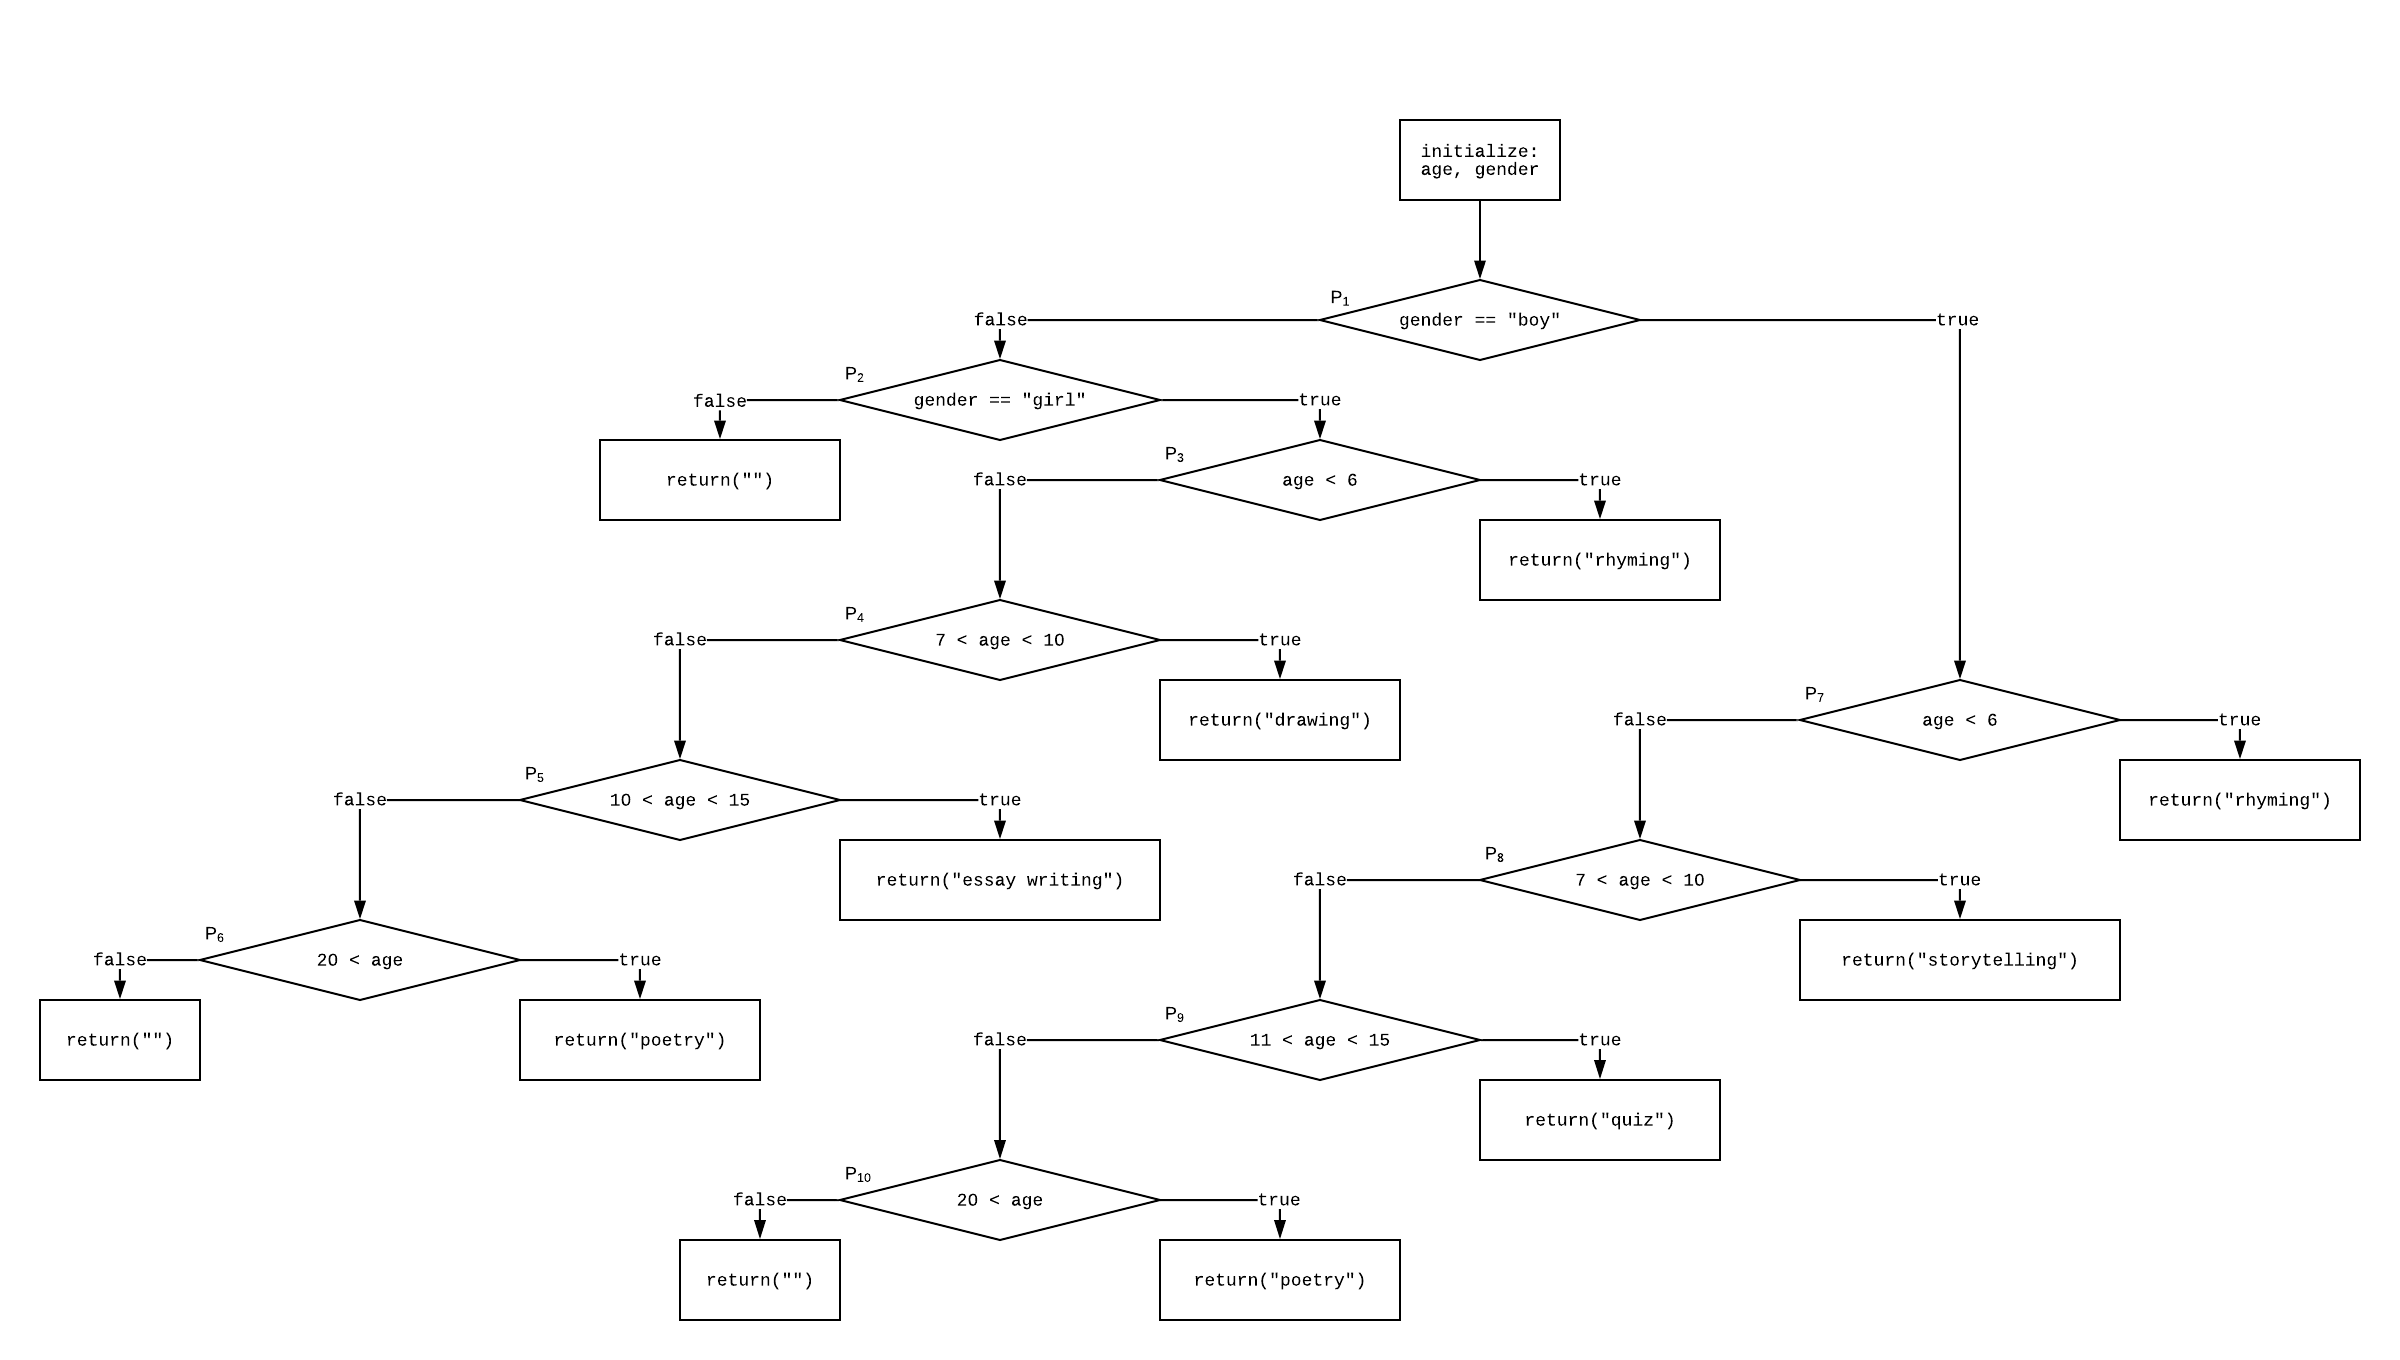
\includegraphics[width=\linewidth]{control-flow.png}
\end{figure}
\newpage

\section{Predicates}
\begin{table}[!htb]
\centering
\begin{tabular}{|l|l|}
\hline
\#  & Predicate        \\ \hline
$P_1$  & gender == "boy"  \\ \hline
$P_2$  & gender == "girl" \\ \hline
$P_3$  & age \textless 6  \\ \hline
$P_{4a}$ & 7 \textless age  \\ \hline
$P_{4b}$ & age \textless 10 \\ \hline
$P_{5a}$ & 10 \textless age \\ \hline
$P_{5b}$ & age \textless 15 \\ \hline
$P_6$  & 20 \textless age \\ \hline
$P_7$  & age \textless 6  \\ \hline
$P_{8a}$ & 7 \textless age  \\ \hline
$P_{8b}$ & age \textless 10 \\ \hline
$P_{9a}$ & 11 \textless age \\ \hline
$P_{9b}$ & age \textless 15 \\ \hline
$P_{10}$ & 20 \textless age \\ \hline
\end{tabular}
\end{table}

\section{Domain Graph}
\begin{tikzpicture}
\begin{axis} [
	axis x line = middle,
	axis y line = middle,
	x=0.6cm,
	xlabel = $age$,
	xlabel style={at=(current axis.right of origin), anchor=west},
	ylabel = $gender$,
	ylabel style={at=(current axis.above origin), anchor=south},
	xmin = 0, xmax = 22,
	ymin = -14, ymax = 14,
	yticklabels={,,}
	]
	\addplot
		[mark=none] coordinates {(0, 0) (0, 5)} 
		node [right] {male};
	\addplot
		[mark=none] coordinates {(0, 0) (0, 1)}
		node [right] {$P_1$, $P_2$};
	\addplot
		[mark=none, color=black, dashed, thick]
		coordinates {(0, 0) (25, 0)};
	\addplot 
		[mark=none, color=black, dashed, thick] 
		coordinates {(6, 0) (6, 10)}
		node [above] {$P_7$};
	\addplot
		[mark=none, color=black, dashed, thick]
		coordinates {(7, 0) (7, 10)}
		node [above] {$P_{8a}$};
	\addplot
		[mark=none, color=black, dashed, thick]
		coordinates {(10, 0) (10, 10)}
		node [above] {$P_{8b}$};
	\addplot
		[mark=none, color=black, dashed, thick]
		coordinates {(11, 0) (11, 10)}
		node [above] {$P_{9a}$};	
	\addplot
		[mark=none, color=black, dashed, thick]
		coordinates {(15, 0) (15, 10)}
		node [above] {$P_{9b}$};
	\addplot 
		[mark=none, color=black, dashed, thick]
		coordinates {(20, 0) (20, 10)}
		node [above] {$P_{10}$};

	\addplot
		[mark=none] coordinates {(0, 0) (0, -5)}
		node [right] {female};
	\addplot 
		[mark=none, color=black, dashed, thick] 
		coordinates {(6, 0) (6, -10)}
		node [below] {$P_3$};
	\addplot
		[mark=none, color=black, dashed, thick]
		coordinates {(7, 0) (7, -10)}
		node [below] {$P_{4a}$};
	\addplot
		[mark=none, color=black, dashed, thick]
		coordinates {(10, 0) (10, -10)}
		node [below] {$P_{4b}$, $P_{5a}$};		
	\addplot
		[mark=none, color=black, dashed, thick]
		coordinates {(15, 0) (15, -10)}
		node [below] {$P_{5b}$};
	\addplot 
		[mark=none, color=black, dashed, thick]
		coordinates {(20, 0) (20, -10)}
		node [below] {$P_{6}$};
\end{axis}
\end{tikzpicture}
\newpage

\section{Test Cases}
Order of tests is ON (on the border), ON, OFF.
\subsection{Predicate $P_1$ gender == ``boy''}
\subsubsection{Boundary Shift - Reduced Domain}
\begin{table}[!htb]
\centering
\begin{tabular}{|l|l|l|l|}
\hline
Test   & Actual Input & Expected Input & Fault Detected \\ \hline
“ ”    & “ ”          & “boy”          & Yes            \\ \hline
“girl” & “girl”       & “boy”          & Yes            \\ \hline
“boy”  & “boy”        & “boy”          & No             \\ \hline
\end{tabular}
\end{table}

\subsubsection{Boundary Shift - Increased Domain}
\begin{table}[!htb]
\centering
\begin{tabular}{|l|l|l|l|}
\hline
Test   & Actual Input & Expected Input & Fault Detected \\ \hline
“ ”    & “ ”          & “girl”         & Yes            \\ \hline
“girl” & “girl”       & “girl”         & No             \\ \hline
“boy”  & “boy”        & “girl”         & Yes            \\ \hline
\end{tabular}
\end{table}

\subsubsection{Boundary Tilt}
\begin{table}[!htb]
\centering
\begin{tabular}{|l|l|l|l|}
\hline
Test   & Actual Input & Expected Input & Fault Detected \\ \hline
“ ”    & “ ”          & “girl”         & Yes            \\ \hline
“girl” & “girl”       & “boy”          & Yes            \\ \hline
“boy”  & “boy”        & “boy”          & No             \\ \hline
\end{tabular}
\end{table}

\subsubsection{Closure Error}
\begin{table}[!htb]
\centering
\begin{tabular}{|l|l|l|l|}
\hline
Test   & Actual Input & Expected Input & Fault Detected \\ \hline
“ ”    & “boy”        & “ ”            & Yes            \\ \hline
“boy”  & “boy”        & “boy”          & No             \\ \hline
“girl” & “girl”       & “girl”         & No             \\ \hline
\end{tabular}
\end{table}
\newpage

\subsection{Predicate $P_2$ gender == ``girl''}
\subsubsection{Boundary Shift - Reduced Domain}
\begin{table}[!htb]
\centering
\begin{tabular}{|l|l|l|l|}
\hline
Test   & Actual Input & Expected Input & Fault Detected \\ \hline
“ ”    & “ ”          & “girl”         & Yes            \\ \hline
“boy”  & “boy”        & “girl”         & Yes            \\ \hline
“girl” & “girl”       & “girl”         & No             \\ \hline
\end{tabular}
\end{table}

\subsubsection{Boundary Shift - Increased Domain}
\begin{table}[!htb]
\centering
\begin{tabular}{|l|l|l|l|}
\hline
Test   & Actual Input & Expected Input & Fault Detected \\ \hline
“ ”    & “ ”          & “boy”          & No             \\ \hline
“boy”  & “boy”        & “boy”          & No             \\ \hline
“girl” & “girl”       & “boy”          & Yes            \\ \hline
\end{tabular}
\end{table}

\subsubsection{Boundary Tilt}
\begin{table}[!htb]
\centering
\begin{tabular}{|l|l|l|l|}
\hline
Test   & Actual Input & Expected Input & Fault Detected \\ \hline
“ ”    & “ ”          & “girl”         & Yes            \\ \hline
“boy”  & “boy”        & “boy”          & No             \\ \hline
“girl” & “girl”       & “girl”         & No             \\ \hline
\end{tabular}
\end{table}

\subsubsection{Closure Error}
\begin{table}[!htb]
\centering
\begin{tabular}{|l|l|l|l|}
\hline
Test   & Actual Input & Expected Input & Fault Detected \\ \hline
“ ”    & “girl”       & “ ”            & Yes            \\ \hline
“girl” & “girl”       & “girl”         & No             \\ \hline
“boy”  & “boy”        & “boy”          & No             \\ \hline
\end{tabular}
\end{table}
\newpage

\subsection{Predicate $P_3$ age \textless 6}
\subsubsection{Boundary Shift - Reduced Domain}
\begin{table}[!htb]
\centering
\begin{tabular}{|l|l|l|l|}
\hline
Test   & Actual Output & Expected Output & Fault Detected \\ \hline
6      & “ ”           & “rhyming”       & Yes            \\ \hline
6.0001 & “ ”           & “rhyming”       & Yes            \\ \hline
5.9999 & “rhyming”     & “rhyming”       & No             \\ \hline
\end{tabular}
\end{table}

\subsubsection{Boundary Shift - Increased Domain}
\begin{table}[!htb]
\centering
\begin{tabular}{|l|l|l|l|}
\hline
Test   & Actual Output & Expected Output & Fault Detected \\ \hline
6      & “ ”           & “ ”             & No             \\ \hline
6.0001 & “ ”           & “ ”             & No             \\ \hline
5.9999 & “rhyming”     & “ ”             & Yes            \\ \hline
\end{tabular}
\end{table}

\subsubsection{Boundary Tilt}
\begin{table}[!htb]
\centering
\begin{tabular}{|l|l|l|l|}
\hline
Test   & Actual Output & Expected Output & Fault Detected \\ \hline
6      & “ ”           & “ ”             & No             \\ \hline
6.0001 & “ ”           & “rhyming”       & Yes            \\ \hline
5.9999 & “rhyming”     & “rhyming”       & No             \\ \hline
\end{tabular}
\end{table}

\subsubsection{Closure Error}
\begin{table}[!htb]
\centering
\begin{tabular}{|l|l|l|l|}
\hline
Test   & Actual Output & Expected Output & Fault Detected \\ \hline
6      & “rhyming”     & “ ”             & Yes            \\ \hline
5.9999 & “rhyming”     & “rhyming”       & No             \\ \hline
6.0001 & “ ”           & “ ”             & No             \\ \hline
\end{tabular}
\end{table}
\newpage

\subsection{Predicate $P_{4a}$ 7 \textless age}
\subsubsection{Boundary Shift - Reduced Domain}
\begin{table}[!htb]
\centering
\begin{tabular}{|l|l|l|l|}
\hline
Test   & Actual Output & Expected Output & Fault Detected \\ \hline
7      & “ ”           & “drawing”       & Yes            \\ \hline
6.9999 & “ ”           & “drawing”       & Yes            \\ \hline
7.0001 & “drawing”     & “drawing”       & No             \\ \hline
\end{tabular}
\end{table}

\subsubsection{Boundary Shift - Increased Domain}
\begin{table}[!htb]
\centering
\begin{tabular}{|l|l|l|l|}
\hline
Test   & Actual Output & Expected Output & Fault Detected \\ \hline
7      & “ ”           & “ ”             & No             \\ \hline
6.9999 & “ ”           & “ ”             & No             \\ \hline
7.0001 & “drawing”     & “ ”             & Yes            \\ \hline
\end{tabular}
\end{table}

\subsubsection{Boundary Tilt}
\begin{table}[!htb]
\centering
\begin{tabular}{|l|l|l|l|}
\hline
Test   & Actual Output & Expected Output & Fault Detected \\ \hline
7      & “ ”           & “drawing”       & Yes            \\ \hline
6.9999 & “ ”           & “ ”             & No             \\ \hline
7.0001 & “drawing”     & “drawing”       & No             \\ \hline
\end{tabular}
\end{table}

\subsubsection{Closure Error}
\begin{table}[!htb]
\centering
\begin{tabular}{|l|l|l|l|}
\hline
Test   & Actual Output & Expected Output & Fault Detected \\ \hline
7      & “drawing”     & “ ”             & Yes            \\ \hline
7.0001 & “drawing”     & “drawing”       & No             \\ \hline
6.9999 & “ ”           & “ ”             & No             \\ \hline
\end{tabular}
\end{table}
\newpage

\subsection{Predicate $P_{4b}$ age \textless 6}
\subsubsection{Boundary Shift - Reduced Domain}
\begin{table}[!htb]
\centering
\begin{tabular}{|l|l|l|l|}
\hline
Test    & Actual Output   & Expected Output & Fault Detected \\ \hline
10      & “ ”             & “drawing”       & Yes            \\ \hline
10.0001 & “essay writing” & “drawing”       & Yes            \\ \hline
9.9999  & “drawing”       & “drawing”       & No             \\ \hline
\end{tabular}
\end{table}

\subsubsection{Boundary Shift - Increased Domain}
\begin{table}[!htb]
\centering
\begin{tabular}{|l|l|l|l|}
\hline
Test    & Actual Output   & Expected Output & Fault Detected \\ \hline
10      & “ ”             & “essay writing” & Yes            \\ \hline
10.0001 & “essay writing” & “essay writing” & No             \\ \hline
9.9999  & “drawing”       & “essay writing” & Yes            \\ \hline
\end{tabular}
\end{table}

\subsubsection{Boundary Tilt}
\begin{table}[!htb]
\centering
\begin{tabular}{|l|l|l|l|}
\hline
Test    & Actual Output   & Expected Output & Fault Detected \\ \hline
10      & “ ”             & “essay writing” & Yes            \\ \hline
10.0001 & “essay writing” & “drawing”       & Yes            \\ \hline
9.9999  & “drawing”       & “drawing”       & No             \\ \hline
\end{tabular}
\end{table}

\subsubsection{Closure Error}
\begin{table}[!htb]
\centering
\begin{tabular}{|l|l|l|l|}
\hline
Test    & Actual Output   & Expected Output & Fault Detected \\ \hline
10      & “drawing”       & “ ”             & Yes            \\ \hline
9.9999  & “drawing”       & “drawing”       & No             \\ \hline
10.0001 & “essay writing” & “essay writing” & No             \\ \hline
\end{tabular}
\end{table}
\newpage

\subsection{Predicate $P_{5a}$ 10 \textless age}
\subsubsection{Boundary Shift - Reduced Domain}
\begin{table}[!htb]
\centering
\begin{tabular}{|l|l|l|l|}
\hline
Test    & Actual Output   & Expected Output & Fault Detected \\ \hline
10      & “ ”             & “essay writing” & Yes            \\ \hline
9.9999  & “drawing”       & “essay writing” & Yes            \\ \hline
10.0001 & “essay writing” & “essay writing” & No             \\ \hline
\end{tabular}
\end{table}

\subsubsection{Boundary Shift - Increased Domain}
\begin{table}[!htb]
\centering
\begin{tabular}{|l|l|l|l|}
\hline
Test    & Actual Output   & Expected Output & Fault Detected \\ \hline
10      & “ ”             & “drawing”       & Yes            \\ \hline
9.9999  & “drawing”       & “drawing”       & No             \\ \hline
10.0001 & “essay writing” & “drawing”       & Yes            \\ \hline
\end{tabular}
\end{table}

\subsubsection{Boundary Tilt}
\begin{table}[!htb]
\centering
\begin{tabular}{|l|l|l|l|}
\hline
Test    & Actual Output   & Expected Output & Fault Detected \\ \hline
10      & “ ”             & “essay writing” & Yes            \\ \hline
9.9999  & “drawing”       & “drawing”       & No             \\ \hline
10.0001 & “essay writing” & “essay writing” & No             \\ \hline
\end{tabular}
\end{table}

\subsubsection{Closure Error}
\begin{table}[!htb]
\centering
\begin{tabular}{|l|l|l|l|}
\hline
Test    & Actual Output   & Expected Output & Fault Detected \\ \hline
10      & “essay writing” & “ ”             & Yes            \\ \hline
10.0001 & “essay writing” & “essay writing” & No             \\ \hline
9.9999  & “drawing”       & “drawing”       & No             \\ \hline
\end{tabular}
\end{table}
\newpage

\subsection{Predicate $P_{5b}$ age \textless 15}
\subsubsection{Boundary Shift - Reduced Domain}
\begin{table}[!htb]
\centering
\begin{tabular}{|l|l|l|l|}
\hline
Test    & Actual Output   & Expected Output & Fault Detected \\ \hline
15      & “ ”             & “essay writing” & Yes            \\ \hline
15.0001 & “ ”             & “essay writing” & Yes            \\ \hline
14.9999 & “essay writing” & “essay writing” & No             \\ \hline
\end{tabular}
\end{table}

\subsubsection{Boundary Shift - Increased Domain}
\begin{table}[!htb]
\centering
\begin{tabular}{|l|l|l|l|}
\hline
Test    & Actual Output   & Expected Output & Fault Detected \\ \hline
15      & “ ”             & “ ”             & No             \\ \hline
15.0001 & “ ”             & “ ”             & No             \\ \hline
14.9999 & “essay writing” & “ ”             & Yes            \\ \hline
\end{tabular}
\end{table}

\subsubsection{Boundary Tilt}
\begin{table}[!htb]
\centering
\begin{tabular}{|l|l|l|l|}
\hline
Test    & Actual Output   & Expected Output & Fault Detected \\ \hline
15      & “ ”             & “ ”             & No             \\ \hline
15.0001 & “ ”             & “essay writing” & Yes            \\ \hline
14.9999 & “essay writing” & “essay writing” & No             \\ \hline
\end{tabular}
\end{table}

\subsubsection{Closure Error}
\begin{table}[!htb]
\centering
\begin{tabular}{|l|l|l|l|}
\hline
Test    & Actual Output   & Expected Output & Fault Detected \\ \hline
15      & “essay writing” & “ ”             & Yes            \\ \hline
14.9999 & “essay writing” & “essay writing” & No             \\ \hline
15.0001 & “ ”             & “ ”             & No             \\ \hline
\end{tabular}
\end{table}
\newpage

\subsection{Predicate $P_6$ 20 \textless age}
\subsubsection{Boundary Shift - Reduced Domain}
\begin{table}[!htb]
\centering
\begin{tabular}{|l|l|l|l|}
\hline
Test    & Actual Output & Expected Output & Fault Detected \\ \hline
20      & “ ”           & “poetry”        & Yes            \\ \hline
19.9999 & “ ”           & “poetry”        & Yes            \\ \hline
20.0001 & “poetry”      & “poetry”        & No             \\ \hline
\end{tabular}
\end{table}

\subsubsection{Boundary Shift - Increased Domain}
\begin{table}[!htb]
\centering
\begin{tabular}{|l|l|l|l|}
\hline
Test    & Actual Output & Expected Output & Fault Detected \\ \hline
20      & “ ”           & “ ”             & No             \\ \hline
19.9999 & “ ”           & “ ”             & No             \\ \hline
20.0001 & “poetry”      & “ ”             & Yes            \\ \hline
\end{tabular}
\end{table}

\subsubsection{Boundary Tilt}
\begin{table}[!htb]
\centering
\begin{tabular}{|l|l|l|l|}
\hline
Test    & Actual Output & Expected Output & Fault Detected \\ \hline
20      & “ ”           & “poetry”        & Yes            \\ \hline
19.9999 & “ ”           & “ ”             & No             \\ \hline
20.0001 & “poetry”      & “poetry”        & No             \\ \hline
\end{tabular}
\end{table}

\subsubsection{Closure Error}
\begin{table}[!htb]
\centering
\begin{tabular}{|l|l|l|l|}
\hline
Test    & Actual Output & Expected Output & Fault Detected \\ \hline
20      & “poetry”      & “ ”             & Yes            \\ \hline
20.0001 & “poetry”      & “poetry”        & No             \\ \hline
19.9999 & “ ”           & “ ”             & No             \\ \hline
\end{tabular}
\end{table}
\newpage

\subsection{Predicate $P_7$ age \textless 6}
\subsubsection{Boundary Shift - Reduced Domain}
\begin{table}[!htb]
\centering
\begin{tabular}{|l|l|l|l|}
\hline
Test   & Actual Output & Expected Output & Fault Detected \\ \hline
6      & “ ”           & “rhyming”       & Yes            \\ \hline
6.0001 & “ ”           & “rhyming”       & Yes            \\ \hline
5.9999 & “rhyming”     & “rhyming”       & No             \\ \hline
\end{tabular}
\end{table}

\subsubsection{Boundary Shift - Increased Domain}
\begin{table}[!htb]
\centering
\begin{tabular}{|l|l|l|l|}
\hline
Test   & Actual Output & Expected Output & Fault Detected \\ \hline
6      & “ ”           & “ ”             & No             \\ \hline
6.0001 & “ ”           & “ ”             & No             \\ \hline
5.9999 & “rhyming”     & “ ”             & Yes            \\ \hline
\end{tabular}
\end{table}

\subsubsection{Boundary Tilt}
\begin{table}[!htb]
\centering
\begin{tabular}{|l|l|l|l|}
\hline
Test   & Actual Output & Expected Output & Fault Detected \\ \hline
6      & “ ”           & “ ”             & No             \\ \hline
6.0001 & “ ”           & “rhyming”       & Yes            \\ \hline
5.9999 & “rhyming”     & “rhyming”       & No             \\ \hline
\end{tabular}
\end{table}

\subsubsection{Closure Error}
\begin{table}[!htb]
\centering
\begin{tabular}{|l|l|l|l|}
\hline
Test   & Actual Output & Expected Output & Fault Detected \\ \hline
6      & “rhyming”     & “ ”             & Yes            \\ \hline
5.9999 & “rhyming”     & “rhyming”       & No             \\ \hline
6.0001 & “ ”           & “ ”             & No             \\ \hline
\end{tabular}
\end{table}
\newpage

\subsection{Predicate $P_{8a}$ 7 \textless age}
\subsubsection{Boundary Shift - Reduced Domain}
\begin{table}[!htb]
\centering
\begin{tabular}{|l|l|l|l|}
\hline
Test   & Actual Output  & Expected Output & Fault Detected \\ \hline
7      & “ ”            & “storytelling”  & Yes            \\ \hline
6.9999 & “ ”            & “storytelling”  & Yes            \\ \hline
7.0001 & “storytelling” & “storytelling”  & No             \\ \hline
\end{tabular}
\end{table}

\subsubsection{Boundary Shift - Increased Domain}
\begin{table}[!htb]
\centering
\begin{tabular}{|l|l|l|l|}
\hline
Test   & Actual Output  & Expected Output & Fault Detected \\ \hline
7      & “ ”            & “ ”             & No             \\ \hline
6.9999 & “ ”            & “ ”             & No             \\ \hline
7.0001 & “storytelling” & “ ”             & Yes            \\ \hline
\end{tabular}
\end{table}

\subsubsection{Boundary Tilt}
\begin{table}[!htb]
\centering
\begin{tabular}{|l|l|l|l|}
\hline
Test   & Actual Output  & Expected Output & Fault Detected \\ \hline
7      & “ ”            & “storytelling”  & Yes            \\ \hline
6.9999 & “ ”            & “ ”             & No             \\ \hline
7.0001 & “storytelling” & “storytelling”  & No             \\ \hline
\end{tabular}
\end{table}

\subsubsection{Closure Error}
\begin{table}[!htb]
\centering
\begin{tabular}{|l|l|l|l|}
\hline
Test   & Actual Output  & Expected Output & Fault Detected \\ \hline
7      & “storytelling” & “ ”             & Yes            \\ \hline
7.0001 & “storytelling” & “storytelling”  & No             \\ \hline
6.9999 & “ ”            & “ ”             & No             \\ \hline
\end{tabular}
\end{table}
\newpage

\subsection{Predicate $P_{8b}$ age \textless 10}
\subsubsection{Boundary Shift - Reduced Domain}
\begin{table}[!htb]
\centering
\begin{tabular}{|l|l|l|l|}
\hline
Test    & Actual Output  & Expected Output & Fault Detected \\ \hline
10      & “ ”            & “storytelling”  & Yes            \\ \hline
10.0001 & “ ”            & “storytelling”  & Yes            \\ \hline
9.9999  & “storytelling” & “storytelling”  & No             \\ \hline
\end{tabular}
\end{table}

\subsubsection{Boundary Shift - Increased Domain}
\begin{table}[!htb]
\centering
\begin{tabular}{|l|l|l|l|}
\hline
Test    & Actual Output  & Expected Output & Fault Detected \\ \hline
10      & “ ”            & “ ”             & No             \\ \hline
10.0001 & “ ”            & “ ”             & No             \\ \hline
9.9999  & “storytelling” & “ ”             & Yes            \\ \hline
\end{tabular}
\end{table}

\subsubsection{Boundary Tilt}
\begin{table}[!htb]
\centering
\begin{tabular}{|l|l|l|l|}
\hline
Test    & Actual Output  & Expected Output & Fault Detected \\ \hline
10      & “ ”            & “ ”             & No             \\ \hline
10.0001 & “ ”            & “storytelling”  & Yes            \\ \hline
9.9999  & “storytelling” & “storytelling”  & No             \\ \hline
\end{tabular}
\end{table}

\subsubsection{Closure Error}
\begin{table}[!htb]
\centering
\begin{tabular}{|l|l|l|l|}
\hline
Test    & Actual Output  & Expected Output & Fault Detected \\ \hline
10      & “storytelling” & “ ”             & Yes            \\ \hline
9.9999  & “storytelling” & “storytelling”  & No             \\ \hline
10.0001 & “ ”            & “ ”             & No             \\ \hline
\end{tabular}
\end{table}
\newpage

\subsection{Predicate $P_{9a}$ 11 \textless age}
\subsubsection{Boundary Shift - Reduced Domain}
\begin{table}[!htb]
\centering
\begin{tabular}{|l|l|l|l|}
\hline
Test    & Actual Output & Expected Output & Fault Detected \\ \hline
11      & “ ”           & “quiz”          & Yes            \\ \hline
10.9999 & “ ”           & “quiz”          & Yes            \\ \hline
11.0001 & “quiz”        & “quiz”          & No             \\ \hline
\end{tabular}
\end{table}

\subsubsection{Boundary Shift - Increased Domain}
\begin{table}[!htb]
\centering
\begin{tabular}{|l|l|l|l|}
\hline
Test    & Actual Output & Expected Output & Fault Detected \\ \hline
11      & “ ”           & “ ”             & No             \\ \hline
10.9999 & “ ”           & “ ”             & No             \\ \hline
11.0001 & “quiz”        & “ ”             & Yes            \\ \hline
\end{tabular}
\end{table}

\subsubsection{Boundary Tilt}
\begin{table}[!htb]
\centering
\begin{tabular}{|l|l|l|l|}
\hline
Test    & Actual Output & Expected Output & Fault Detected \\ \hline
11      & “ ”           & “quiz”          & Yes            \\ \hline
10.9999 & “ ”           & “ ”             & No             \\ \hline
11.0001 & “quiz”        & “quiz”          & No             \\ \hline
\end{tabular}
\end{table}

\subsubsection{Closure Error}
\begin{table}[!htb]
\centering
\begin{tabular}{|l|l|l|l|}
\hline
Test    & Actual Output & Expected Output & Fault Detected \\ \hline
11      & “quiz”        & “ ”             & Yes            \\ \hline
11.0001 & “quiz”        & “quiz”          & No             \\ \hline
10.9999 & “ ”           & “ ”             & No             \\ \hline
\end{tabular}
\end{table}
\newpage

\subsection{Predicate $P_{9b}$ age \textless 15}
\subsubsection{Boundary Shift - Reduced Domain}
\begin{table}[!htb]
\centering
\begin{tabular}{|l|l|l|l|}
\hline
Test    & Actual Output & Expected Output & Fault Detected \\ \hline
15      & “ ”           & “quiz”          & Yes            \\ \hline
15.0001 & “ ”           & “quiz”          & Yes            \\ \hline
14.9999 & “quiz”        & “quiz”          & No             \\ \hline
\end{tabular}
\end{table}

\subsubsection{Boundary Shift - Increased Domain}
\begin{table}[!htb]
\centering
\begin{tabular}{|l|l|l|l|}
\hline
Test    & Actual Output & Expected Output & Fault Detected \\ \hline
15      & “ ”           & “ ”             & No             \\ \hline
15.0001 & “ ”           & “ ”             & No             \\ \hline
14.9999 & “quiz”        & “ ”             & Yes            \\ \hline
\end{tabular}
\end{table}

\subsubsection{Boundary Tilt}
\begin{table}[!htb]
\centering
\begin{tabular}{|l|l|l|l|}
\hline
Test    & Actual Output & Expected Output & Fault Detected \\ \hline
15      & “ ”           & “ ”             & No             \\ \hline
15.0001 & “ ”           & “quiz”          & Yes            \\ \hline
14.9999 & “quiz”        & “quiz”          & No             \\ \hline
\end{tabular}
\end{table}

\subsubsection{Closure Error}
\begin{table}[!htb]
\centering
\begin{tabular}{|l|l|l|l|}
\hline
Test    & Actual Output & Expected Output & Fault Detected \\ \hline
15      & “quiz”        & “ ”             & Yes            \\ \hline
14.9999 & “quiz”        & “quiz”          & No             \\ \hline
15.0001 & “ ”           & “ ”             & No             \\ \hline
\end{tabular}
\end{table}
\newpage

\subsection{Predicate $P_{10}$ 20 \textless age}
\subsubsection{Boundary Shift - Reduced Domain}
\begin{table}[!htb]
\centering
\begin{tabular}{|l|l|l|l|}
\hline
Test    & Actual Output & Expected Output & Fault Detected \\ \hline
20      & “ ”           & “poetry”        & Yes            \\ \hline
19.9999 & “ ”           & “poetry”        & Yes            \\ \hline
20.0001 & “poetry”      & “poetry”        & No             \\ \hline
\end{tabular}
\end{table}

\subsubsection{Boundary Shift - Increased Domain}
\begin{table}[!htb]
\centering
\begin{tabular}{|l|l|l|l|}
\hline
Test    & Actual Output & Expected Output & Fault Detected \\ \hline
20      & “ ”           & “ ”             & No             \\ \hline
19.9999 & “ ”           & “ ”             & No             \\ \hline
20.0001 & “poetry”      & “ ”             & Yes            \\ \hline
\end{tabular}
\end{table}

\subsubsection{Boundary Tilt}
\begin{table}[!htb]
\centering
\begin{tabular}{|l|l|l|l|}
\hline
Test    & Actual Output & Expected Output & Fault Detected \\ \hline
20      & “ ”           & “poetry”        & Yes            \\ \hline
19.9999 & “ ”           & “ ”             & No             \\ \hline
20.0001 & “poetry”      & “poetry”        & No             \\ \hline
\end{tabular}
\end{table}

\subsubsection{Closure Error}
\begin{table}[!htb]
\centering
\begin{tabular}{|l|l|l|l|}
\hline
Test    & Actual Output & Expected Output & Fault Detected \\ \hline
20      & “poetry”      & “ ”             & Yes            \\ \hline
20.0001 & “poetry”      & “poetry”        & No             \\ \hline
19.9999 & “ ”           & “ ”             & No             \\ \hline
\end{tabular}
\end{table}
\newpage

\end{document} 